\chapter{Background}
This chapter mainly contains relevant background theory on blockchains. The chapter starts off with a very basic introduction to microgrids. Related work on the subject is presented at the end of the chapter. 

\section{Microgrids}
A microgrid is a local power grid that may or may not be connected to the main grid. The microgrid can either work as an extension of the main power grid, or operate in \enquote{island mode} and function autonomously. A formal definition of a microgrid is as follows: 

\enquote{\textit{A Microgrid is a group of interconnected loads and distributed energy resources within clearly defined electrical boundaries that acts as a single controllable entity with respect to the grid}} \cite{micro_securicon}.

Microgrids usually include renewable energy sources, such as wind generators, small hydro power generation, and photovoltaic solar panels, that are locally grouped together. Microgrids may also include generators and batteries to ensure reliability \cite{general_microgrid}. By placing power generation and power usage closer together, efficiency will be increased and transmission losses reduced \cite{Microgrid_konashevych}. 

A key benefit of the microgrid, is the ability of being self-sufficient in case of emergencies that cause blackouts. By disconnecting from the grid, the locale area powered by the microgrid can operate for days without any connection to the main grid. This happened, for instance, in New York during hurricane Sandy in 2012 \cite{sandy}. The city was without power for several days, but hospitals and other key facilities could operate due to microgrids. 

Places that are not connected to the main grid have very expensive solutions for getting power. This can typically be rural places or islands. They may also benefit from microgrids. The ability to operate in island-mode will provide better electricity services at a lower cost than e.g. importing diesel \cite{abb}.

\subsection{Electrical Transmission}
In microgrids, just like in the traditional power grid, there is no way of telling where consumed electrons are actually generated. Once a power plant or another power producer put electricity in to the grid, the electrons from all sources are mixed together before they are transferred to consumers \cite{timneypower}. The electricity sources are indistinguishable. In a microgrid, this means that even if producer A has a contract with consumer B to deliver electricity, consumer B is not necessarily using the electrons that producer B has generated. If producer C is also generating electricity to the gird, there is a chance that consumer B is actually consuming the electrons from producer C. Electrons in the grid always flow from source (generators) to sink (loads), where electricity is being consumed \cite{tracing}. 

\section{Introduction to Blockchain} \label{blockchain_basics}
A blockchain is a decentralized ledger, distributed over a network of nodes. Transactions in the network are stored in blocks which are linked together as a chain, creating the blockchain. It was first introduced by Satoshi Nakamoto with the Bitcoin application \cite{Nakamoto_bitcoin}.

The blockchain is primarily used to transfer assets between users. In contrast to previous transaction methods, there is no need for trust between the participants of the transaction, nor the need of a trusted third-party institution, like a bank or government. The trust lies in the system, and the mathematical functions behind it, and not the individual participants \cite{Nofer}. Due to the decentralization of the network, there is no single-point-of-failure, as the database is duplicated on every node of the network.

The following description of the blockchain technology is based on the Bitcoin blockchain proposed in Nakamotos whitepaper from 2008\cite{Nakamoto_bitcoin}. Many of the features from the Bitcoin blockchain hold true for most blockchains. However, there are many variations of blockchain implementations, due to public/private configurations, consensus models etc. These differences will be described later in the chapter.

When a node transfers an asset to another node, it creates a transaction. The transaction contains: one or more inputs; one or more outputs; and a digital signature. In Bitcoin, an input is a previously received and unspent output, containing the amount of bitcoins. Multiple inputs can be added together to create a larger transaction. The inputs are used completely, so if the amount does not add up to the wanted output, multiple outputs can be used so that the change is sent back to the owner. This is because transactions must reference an output, and each output can only be referenced once. Thus, the exact ownership of every asset can be pinpointed to a user in the network, based on the previous transactions. In order for a transaction to occur, it must be proved that the asset has not been previously spent by the current owner. Thus, there is no way to double spend assets.

Transactions are validated through digital signatures, proving the authenticity of a message, by using public and private keys. Each node can obtain a random private key, and a corresponding public key derived from the private key. If node A wants to send a Bitcoin to node B, it must use B's public key, which acts as the address to B's Bitcoin wallet. Node A creates a digital signature of the transaction with its private key. The validity of the transaction can then be confirmed using A's public key. When the transaction is confirmed, the Bitcoin can only be spent by the person in possession of the private key corresponding to B's public key. This 
transaction is illustrated in figure \ref{fig:sign}. The use of digital signatures ensures that transactions can traverse the network without being altered, as even the smallest change will cause a signature to no longer be valid. 

\begin{figure}[!htb]
\centering
	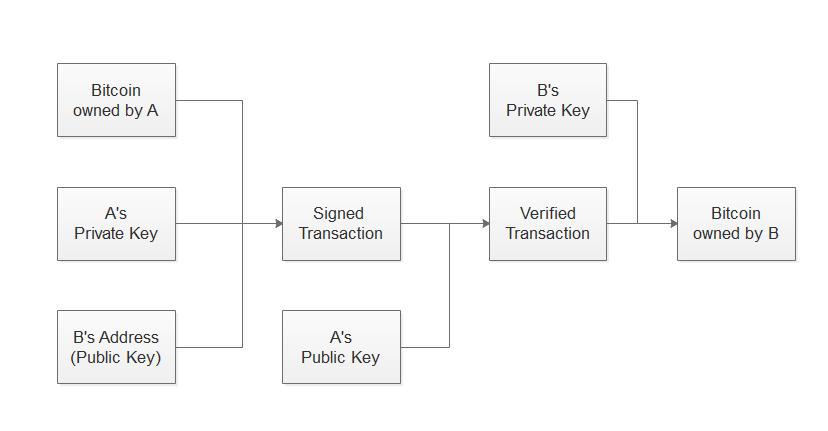
\includegraphics[width=1\textwidth]{Images/sign}
	\caption{Digital signature in Bitcoin transaction.}
	\label{fig:sign}
\end{figure}

A miner stores multiple pending and unconfirmed transaction together to create a block. The block consists of the transactions, as well as the block header. The block header usually contains: a reference to the previous block in the chain, namely the hash of the previous block; a timestamp for when the new block is created; and a nonce and a target used to calculate the hash of the new block. 

When the hash of the new block is found, the block is broadcasted to the rest of the network. Every node on the network validates the block, before they start working on the next block. Validation is an easy task, once the hash is found. If several miners find the solution to the next block at the exact same time, a fork is created. This sequence is illustrated in figure \ref{fig:blocks}
\begin{figure}[!htb]
\centering
	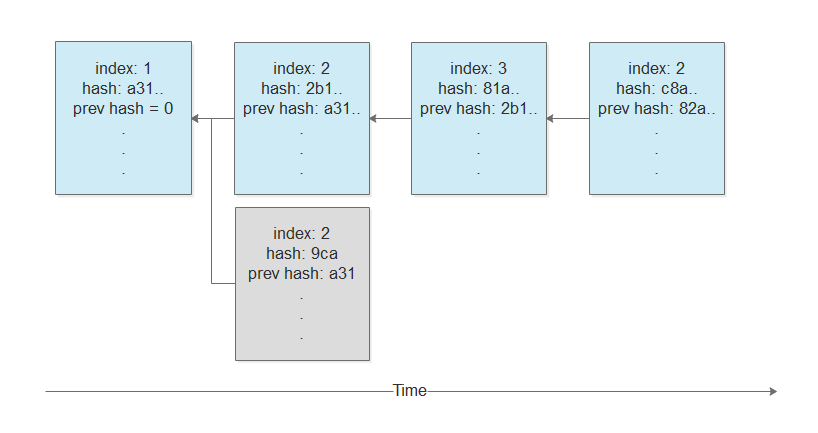
\includegraphics[width=1\textwidth]{Images/blocks}
	\caption{Connection between blocks.}
	\label{fig:blocks}
\end{figure}

A fork means that there exists  two (or more) different versions of the blockchain in the network. Due to network latencies, nodes in the network will receive different broadcasted messages at different times. Therefore, nodes might have different versions of the blockchain. The miners start working on the next block based on the one they received first, while storing the other version in case that fork becomes longer \cite{Nakamoto_bitcoin}. The fork is resolved when one side of the fork becomes longer than the other(s), which will most likely happen when the next block is created. The side with the longest chain always wins because it is backed by the most work. All the nodes in the network immediately look to the longest chain as the valid version of the blockchain. The transactions in the discarded block go back into the pool of the pending transactions, waiting to be mined in a block. Once a transaction is part of the blockchain, it is irreversible. Due to the hash functions, even the slightest alteration in a transaction will be detected, and the transaction will be deemed as non-valid. Thus, a transaction cannot be changed or reverted once it is part of the blockchain. There is however some need for caution. As previously mentioned, transactions in discarded blocks go back to being unconfirmed. If the other side of the fork contains a transaction attempting to double spend the asset, the initial transaction might no longer be valid. 

Say, for instance node A sends two bitcoins to node B, while also sending the same two bitcoins to itself, only one of these transactions can be valid. Once a transaction is stored in the blockchain, the two bitcoins are referenced as a new unspent output, and the other transaction is no longer valid. This is intentional behavior in the blockchain, as it solves the problem of double spending which is usually what a trusted third-party, e.g. a bank, is needed for. The problem occurs when there is a fork. If node B receives the bitcoins as a payment for some goods, and ships the goods once the transaction is part of the blockchain, while node A is simultaneously working on another fork in the blockchain containing the transaction sending the two bitcoins to itself, node B will lose the payment for the goods if the fork node A is working on becomes longer. It is therefore a good policy to wait until the block containing the transactions has multiple successors before asserting the transaction final.


\section{Blockchain Taxonomy}
This section details the taxonomy of blockchains, in particular how they are governed and the level of authorization needed in the different classifications.
Blockchains are usually divided into three different categories, depending on the way they are governed \cite{Ethereum_pub_priv, taxonomy, Zheng_overview}.

\begin{itemize}
\item Public blockchains, like Bitcoin, is a blockchain where anyone is free to participate, and is completely decentralized.
\item Private blockchains are more centralized with e.g. a single organization controlling the blockchain.
\item A consortium blockchain is a hybrid between the two, where participants must be authorized, but there is no single, central authority controlling it. It is also described as \enquote{\textit{[...] a traditional centralized system with a degree of cryptographic auditability attached}}\cite{Ethereum_pub_priv}.
\end{itemize}

Authorization in the blockchain depends on whether they are  permissioned or permissionless. Permissionless blockchains are open to anyone, while permissioned blockchains require approval from the owner or members to join. Public blockchains are categorized as permissionless, while private and consortium blockchains fall under the category of permissioned.

The characteristics of public, private and consortium blockchains are summarized in table \ref{table:private}.

\begin{table}[ht] 
 
 \centering
 \captionof{table}{Comparison between public, private, and consortium blockchains.}
  \label{table:private} 
  \begin{center}
  \scalebox{0.90}{
  \begin{tabular}{*{4}{|c}|}
  
  \hline
  & Public & Private & Consortium\\
  \hline
  Consensus & All miners & One organization & Some nodes \\
  \hline
  Authorization & Permissionless & Permissioned & Permissioned \\
  \hline  
  Performance & Slow & Very fast & Fast\\
  \hline
  Security & Nearly impossible & Could be altered  & Could be altered\\
  & to alter & & \\
  \hline
  Centralization & No & Yes & Partially \\
  \hline  
  Computational & Costly & Cheap & Depends on consensus \\
  expensiveness & & & \\
  \hline  
  Area of use & Crypto-currency & One organization & Several organization \\
  & & & with some trust \\
  \hline
  Anonymity & Yes & No & No \\
  \hline

\end{tabular}}
\end{center}
\end{table}

In conclusion, the type of blockchain most beneficial for each application will vary from industry to industry and from application to application. Public blockchains are most beneficial for individual users, as there is no need for trusted third-parties or trust between users. Private and consortium blockchains are more beneficial to organizations or companies, as they lower cost and increase speed of transactions.


%\subsubsection*{Public Blockchains}
%A public blockchain is completely unregulated. It is open to anyone to read, and transactions are completely transparent. It is also open to anyone wishing to make transactions or participate in the consensus process for validating blocks - making it fully decentralized \cite{Ethereum_pub_priv}. 

%Public blockchains rely heavily on cryptoeconomics for security in an otherwise low-trust environment \cite{cryptoeconomics}.Cryptoeconomics is described as \enquote{\textit{a combination of economic incentives and cryptographic verification using mechanisms such as proof of work or proof of stake, following a general principle that the degree to which someone can have an influence in the consensus process is proportional to the quantity of economic resources that they can bring to bear}} \cite{Ethereum_pub_priv}. 

%Additional benefits of the openness of a blockchain includes the resistance to censorship. A single node or a group of nodes, provided they do not control a big enough (usually 51 \% depending on the consensus model) portion of the network, cannot keep transactions out of the blockchain. 

%https://www.linkedin.com/pulse/difference-between-private-public-consortium-collin-thompson/ extremely secure, but slow and wasteful


%\subsubsection*{Private Blockchains}
%Private blockchains requires trust between peers, usually in the form of a \enquote{middleman} who owns the blockchain and is also in charge of the consensus process.

%Some reasons why this might be desirable is e.g. when there is the need to revert transactions. Say, for instance, that in a blockchain 

%Reverse verified transactions in event of e.g. system error, fraudulent activity, mistake in recipient address. 
%Reduced access lowers risk of outsider attack    
%Benefits of blockchain require some for of mistrust between users, otherwise a shared database might be a better solution
%No single point of failure, as not dependent on one single computer
%Cheaper due to no transaction fees 
%Little or no chance of 51\% attacks
%\cite{Ethereum_pub_priv} : a fully private blockchain is a blockchain where write permissions are kept centralized to one organization. Read permissions may be public or restricted to an arbitrary extent. Likely applications include database management, auditing, etc. internal to a single company, and so public readability may not be necessary in many cases at all, though in other cases public auditability is desired. the fundamental value of blockchains in a fully private context, aside from the replicated state machine functionality, is cryptographic authentication, and there is no reason to believe that the optimal format of such authentication provision should consist of a series of hash-linked data packets containing Merkle tree roots. Private advantages: possible to change rules and revert transactions, known validators – no risk of 51% attack, cheaper transactions, easier consensus algorithms leading to shorter block times, restricted read permissions lead to greater privacy. 
%\cite{Thompson_private} "Private blockchains provide higher leveles of error checking and transaction validity than regular shared databases." "Distributed ledgers are shared databases with access protection rights, with defined rules on what types of changes can be performed by what entities." the security promises of distributed ledgers and private blockchains are only as good as the honesty of the entities validating the transactions. 

%\subsubsection*{Consortium Blockchains}

%A consortium blockchain is a blockchain where the consensus process is controlled by a pre-selected set of nodes; for example, one might imagine a consortium of 15 financial institutions, each of which operates a node and of which 10 must sign every block in order for the block to be valid. The right to read the blockchain may be public, or restricted to the participants, and there are also hybrid routes such as the root hashes of the blocks being public together with an API that allows members of the public to make a limited number of queries and get back cryptographic proofs of some parts of the blockchain state. These blockchains may be considered partially decentralized. \cite{Ethereum_pub_priv}


\section{Consensus Models} 
Consensus models are important in distributed systems, in order to reach distributed agreement and maintain a correct and concise version of the shared ledger between the nodes \cite{Li_pos}. 
There are two different types of fault-tolerance in consensus mechanisms. Fail-stop fault-tolerance means that the system is able to perform correct behavior if it is able to detect nodes that have failed. Byzantine fault-tolerance (BFT) means that the system performs correct behavior even if there are malicious nodes that intentionally try to cause failures in the system. BFT protocols are designed to be a solution to the Byzantine Generals problem (BGP) \cite{byzantine_lamport}. Roughly explained, the BGP is a compliance problem where generals in the Byzantine army must agree upon whether to attack or retreat, using only messages, even if there is a traitor among them.


\subsection{Proof of Work}
Proof of Work (PoW) is the consensus model presented by Nakamoto in the Bitcoin white paper \cite{Nakamoto_bitcoin}, and the most commonly used consensus protocol in blockchains CITE. In the PoW consensus model, nodes are required to put a certain amount of work into creating new blocks to avoid DDoS-attacks and to make it harder for malicious nodes to hijack the blockchain. The required work consists of solving a computationally expensive cryptographic problem. Each new block has a unique hash based. The problem consists of combining this hash with a variable called nonce, to find a hash that is less than a given target (e.g. a 256 bit hash containing x significant zeros). While the proof is somewhat difficult to find, it is very fast and easy to verify by the rest of the network.

By lowering the target value, the problem can be adjusted to be more difficult. The amount of work required is exponential to the number of significant zero bits. This implies that untrustworthy peers wanting to modify past blocks have to work much harder than peers adding new blocks, due to the work required to redo already mined blocks. This can be seen in figure \ref{fig:bitcoin_security}

\begin{figure}[ht]
    \centering
    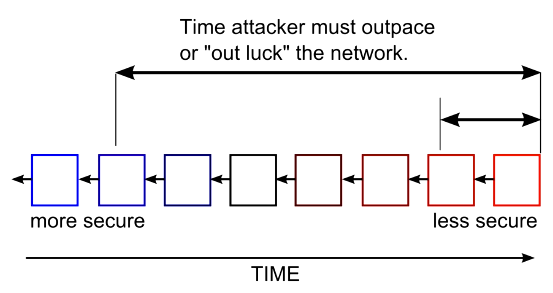
\includegraphics[width=1\textwidth]{Images/bitcoin_security}
    \caption{Transactions in blocks are in less danger of being altered as more time passes \cite{Driscoll}}
    \label{fig:bitcoin_security}
\end{figure}

Nodes working on fining these proofs are called miners, and receive some form of rewards for finding the correct proofs (e.g. a certain amount of the cryptocurrency or transaction fees). Special Application Specific Integrated Circuits (ASIC) computers are created for mining. These computers solve the hash problems at higher rates and with less energy consumption than normal computers \cite{mining}. By letting anyone participate as a miner it is ensured that the network has complete decentralization.

As described by Nakamoto, PoW is also a method for ensuring that a majority always controls the blockchain \cite{Nakamoto_bitcoin}: \enquote{\textit{If the majority were based on one-IP-address-one-vote, it could be subverted by anyone able to allocate many IPs. Proof-of-work is essentially one-CPU-one-vote}}.  The longest chain reflects the most proof-of-work and, thus represented by the majority in the network.

Some of the major problems related to PoW come from the latency and vast amounts of energy required to mine new blocks. As of May 2018, the Bitcoin blockchain consumed more energy than the entire country of Switzerland \cite{bitcoin_energy}, as seen in figure \ref{fig:bitcoin_energy}. 

\begin{figure}[ht]
    \centering
    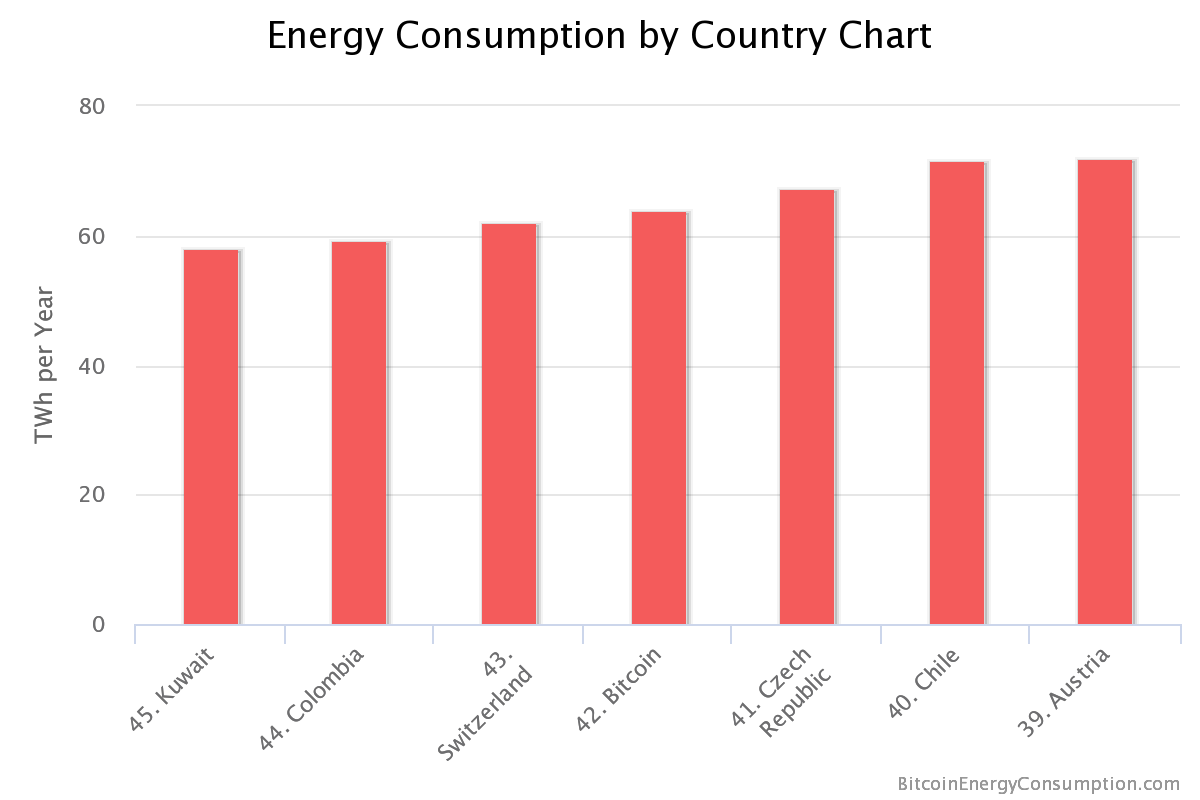
\includegraphics[width=1\textwidth]{Images/bitcoin_energy}
    \caption{Bitcoins energy consumption index relative to countries in the world \cite{bitcoin_energy}}
    \label{fig:bitcoin_energy}
\end{figure}


Nakamoto shows that the probability of an attacker altering a block decreases as more blocks are added on top of it \cite{Nakamoto_bitcoin}. However, the probability never reaches zero. An example of this is the 51 \% attack, where a group wishing to attack the blockchain gains 51 \% of the computation power, and thus is in control of the blockchain. 

PoW ensures that the blockchain eventually reaches consensus. Due to the possibilities of forks in the chain, it might take some time for the network to agree on the final version of the ledger. This results in slow transaction time with only 7 transactions per second, compared to VISAs throughput of 10 000 transactions per second \cite{understanding_consensus}. 

\subsection{Proof of Stake}
Proof of Stake (PoS) was created to solve the energy problem of PoW \cite{understanding_consensus, Zheng_overview}. Nodes are chosen to participate in the consensus process in a deterministic manner, based on the amount of stake they have in the system. This means that if a node, or stakeholder has 10 times more assets in the network than another node, it is 10 times more likely \cite{ethereum_wiki} to be chosen to forge new blocks and hence receive a reward. The reward in PoS comes from transaction fees, as there are no new coins to be mined, or created, since all coins exists from the start of the blockchain. 

The creator of a new block puts his or her own coins at stake. This means that if they produce a block containing fraudulent transactions, they lose their stake. After putting up the stake, the node becomes part of the validation process. Due to their stake in the block, they are incentivized to only validated the correct transactions. The problem occurs when a validator has very little, or nothing, at stake. It is more economical profitable to vote on multiple blocks, supporting multiple chains in order to maximize expected rewards \cite{understanding_consensus, Li_pos}. This problem is known as the nothing-at-stake problem. Ethereum, who is currently using PoW but plan to change to PoS in a future release, proposed a solution to the nothing-at-stake problem by penalizing validators who vote for the wrong block \cite{ethereum_wiki}. 

A major problem with this model is that the rich get richer, due to the selection process favoring nodes with more stake. This, in turn, implies that the network will be more centralized over time. However, it can be argued \cite{rich2} that PoW favors the rich even more, as it is more expensive to purchase hardware required for mining and electricity costs, than buying coins in the blockchain to be more likely to participate in the validation process \cite{rich}.

\subsection{Raft}
Raft is a partially asynchronous, leader based consensus algorithm for managing replicated logs across a distributed system \cite{raft}. Raft was designed to be a more understandable alternative to Paxos \cite{paxos}. The algorithm was first proposed by Onargo et al \cite{raft}. Following is a description of the algorithm.

The Raft algorithm consists of three main parts: \textbf{leader election}, \textbf{log replication}, and \textbf{safety}. Any node participating in the consensus process is in one of three states: leader, follower, or candidate.

\begin{figure}[ht]
    \centering
    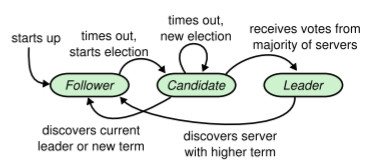
\includegraphics[width=1\textwidth]{Images/raft_state}
    \caption{Server states. \cite{raft}}
    \label{fig:raft_state}
\end{figure}

Time is divided into terms in Raft. Each term is of arbitrary length, depending on the operation of the leader. Each term starts with a \textbf{leader election}. If a node has not heard anything from a leader after a certain amount of time, it becomes a candidate and request votes from other nodes in the network. There are three possible outcomes for a candidate:

\begin{enumerate}
\item The candidate receives a majority of votes and becomes leader.
\item The candidate receives a message from another node claiming to be the leader. The candidate then steps down and becomes a follower.
\item If the candidate does not receive a majority, e.g. due to a split vote, it will start a new term and a new election.
\end{enumerate}

The algorithm guarantees that the following properties are true at all times, thus ensuring consensus: 
\begin{itemize}
\item \enquote{\textbf{Election Safety:} \textit{at most one leader can be elected in a given term}}
\item \enquote{\textbf{Leader Append-Only:} \textit{a leader never overwrites or deletes entries in its log; it only appends new entries}}
\item \enquote{\textbf{Log Matching:} \textit{if two logs contain an entry with the same index and term, then the logs are identical in all entries up through the given index}}
\item \enquote{\textbf{Leader Completeness:} \textit{if a log entry is committed in a given term, then that entry will be present in the logs of the leaders for all higher-numbered terms}}
\item \enquote{\textbf{State Machine Safety:} \textit{if a server has applied a log entry at a given index to its state machine, no other server will ever apply a different log entry for the same index}}
\end{itemize}

When the system operates under normal conditions, there is exactly one server and all other nodes are followers. The followers are passive, and only respond to requests from leaders or candidates through Remote Procedure Calls (RPC). Each \textbf{log entry} consists of an index and a term, as well as some data. If two entries in different logs have the same index and term, all entries up to that point are guaranteed to be identical. Leader cannot overwrite any committed log entries, only append new entries. 

\textbf{Safety} is ensured in Raft by putting restrictions on which nodes can become leaders. A candidate must include all previous committed entries in its log, in order to become a leader. The leader also ensures that any followers missing entries are brought up to date. 

In Bitcoin, and other blockchains with PoW consensus, transactions are never finalized, in the sense that they can become part of a fork. As time passes and more blocks are created, a transaction is less likely to be part of a fork. In Raft however, transactions are finalized when the block becomes part of the blockchain. Due to the leader configuration and validation prior to the blockchain, forks do not occur. 

Raft is not a BFT consensus protocol, it is only fail-stop fault-tolerant. All nodes participating in the consensus are assumed to be trusted, meaning that there are no Byzantine faulty nodes. 


\subsection{Practical Byzantine Fault Tolerance} 

A Byzantine fault-tolerant algorithm is one that can tolerate Byzantine faults that usually occur in network systems with multiple nodes communicating. These types of faults include:

\begin{itemize}
\item Messages lost due to network failures.
\item Messages corrupted through malicious nodes.
\item Messages compromised through man-in-the-middle. attacks.
\item Hardware or software failures.
\item Messages from nodes without permission to join the network.
\item Arbitrary behavior.
\end{itemize}

The Byzantine Generals problem was first proposed and solved by Lamport et al. \cite{byzantine_lamport}. However, the solutions presented in the paper are expensive in regard to time and message overhead, thus making it impractical to use in real systems. A solution to this problem was proposed by Castro et.al \cite{pbft} with their new \textit{Practical Byzantine Fault Tolerance} (PBFT) algorithm.

The PBFT algorithm states that the system is able to make progress with \textit{f} faulty nodes, if the total number of nodes \textit{n}, is
\begin{equation*}
n = 3f + 1
\end{equation*}

Out of the n nodes in the consensus model, one is the primary, which receives requests from the client, and the rest of the nodes are replicas. After receiving a request, the primary initiates a three-phase protocol, (pre-prepare, prepare, and commit) to ensure consensus. Results from all replicas are sent to the client, who in turn accepts the result if there are f+1 identical replies. In the pre-prepare phase, the request is given a unique sequence number, which the replicas agree on in the prepare phase. The commit phase establishes total order across views. The order of communication in the three-phase protocol can be seen in figure \ref{fig:pbft}.

\begin{figure}[htb]
    \centering
    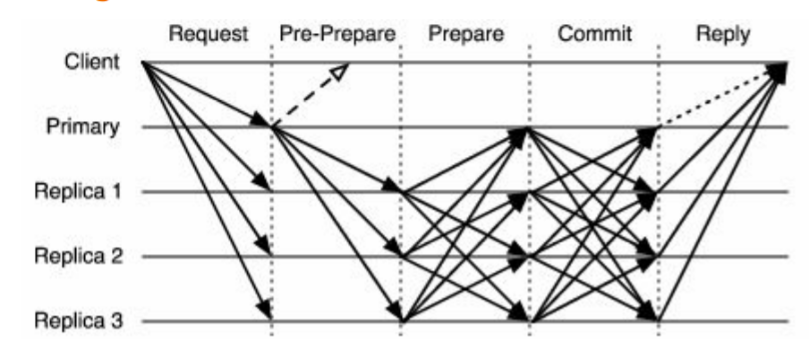
\includegraphics[width=1\textwidth]{Images/pbft}
    \caption{Three-phase protocol for consensus in PBFT \cite{pbft}.}
    \label{fig:pbft}
\end{figure}
 
Hyperledger Fabric provides consensus as a modular component in the system, supporting various kinds of consensus models. One module utilizes PBFT to order transactions in the system, thus ensuring that all peers have the same list of transactions in their ledger \cite{hyperledger, hyperledger_pbft}. 

\subsection{Summery of Consensus Models}
\begin{table}[!ht] 
  
  \centering
  \captionof{table}{Consensus models}
  \label{tab:consensus}  
  \begin{center}
  \scalebox{0.85}{
  \begin{tabular}{*{5}{|c}|}
  
  \hline
  Protocol & PoW & PoS & Raft & PBFT \\
  \hline
  Requires crypto & Yes & Yes & No & No \\
  \hline
  Leader & No & No & Yes & Yes \\
  \hline
  Pros	& Decentralized & Energy efficient & & High throughput \\
        & & & & Low cost \\
  \hline
  Cons & Slow throughput & Nothing at stake & Not BFT & Semi-trusted \\
  	   & Energy inefficient & & & \\
 \hline
 Implementations & Bitcoin & Peercoin & & Hyperledger \\
 				 & Ethereum & Ethereum & & Tendermint\\
 \hline
\end{tabular}}
\end{center}
\end{table}

%SUM UP TABLE, discuss scalability. Both Raft and PBFT require a lot of message passing which does not scale well when the system becomes large. 

This is perhaps the most challenging aspect in order to create a blockchain. Different types of blockchains require different types of consensus models.  
At this point, no single best consensus model exists. Limitations and restrictions are present in regard to power consumption, scaling, security and transaction speed. These challenges will be further discussed in the following section. 

%\section{Security and Weaknesses in Blockchain technology} \label{security}
%51 percent attacks https://learncryptography.com/cryptocurrency/51-attack - older blocks more secure, newer blocks more vulnerable to double spending attacks achieved by mining faster than the rest of the network
%Scaling
%Speed
%Energy consumption
%No possibility to revert transactions in public
%Sybil attacks
%Double spending and rejecting transaction (51%)

%\cite{Chakravarty_guide} : Public Blockchain, which ensures anonymity in identity but transparency in transactions. However, maintaining both anonymity and transactional transparency comes at a cost — it lowers the bandwidth between nodes and the entire blockchain must be duplicated by all nodes locally to be aware of the current state of the chain. 

%Centralized the mining to countries with cheap electricity - vulnerable to changes in policy on electricity subsidies %\cite{hbr_safe}


%\cite{economist_chain}: cap the size of a block at one megabyte, or about 1,400 transactions, it can handle only around seven transactions per second, compared to the 1,736 a second Visa handles in America. Blocks could be made bigger; but bigger blocks would take longer to propagate through the network, worsening the risks of forking

%\cite{Zheng_overview} : due to the original restriction of block size and the time interval used to generate a new block, the Bitcoin blockchain can only process nearly 7 transactions per second, which cannot fulfill the requirement of processing millions of transactions in real-time fashion. Meanwhile, as the capacity of blocks is very small, many small transactions might be delayed since miners prefer those transactions with high transaction fee

%\cite{Zheng_overview} :  blockchain cannot guarantee the transactional privacy since the values of all transactions and balances for each public key are publicly visible. Besides, the recent study [41] has shown that a user’s Bitcoin transactions can be linked to reveal user’s information. Moreover, Biryukov et al. [11] presented a method to link user pseudonyms to IP addresses even when users are behind Network Address Translation (NAT) or firewall. Selfish mining and stubborn mining

%https://arxiv.org/pdf/1703.03779.pdf ponzi on ethereum
\section{Blockchains and Their Applications}
Numerous blockchains have been created since the Bitcoin blockchain was published. Many blockchains, like Bitcoin, are based around crypto-currency. However, there are several blockchain with other purposes than being purely a crypto-currency, such as the Ethereum blockchain. Some of these blockchains will be discussed in this section.

\subsection{Bitcoin}
How Bitcoin works, was roughly described in section \ref{blockchain_basics}. This section will discuss what Bitcoin is used for and in what applications it is beneficial for. Bitcoin is first and foremost a crypto-currency blockchain, so the applications are financial.

The Silk Road drug market \cite{silk}, albeit illegal, is perhaps the field where Bitcoin provided the most convenience for its users, before it was shut down by the FBI in 2013. By using Bitcoins as payment, the marketplace ensured anonymous drug trading. In its 2.5 years of operation, the dark web market had sales worth over \$ 1 billion \cite{Ethereum_visions}.

Another major advantage of Bitcoin is transferring money abroad \cite{wirex}. Compared to traditional transfers between banks which are both costly (on average 7.45\% \cite{world_bank_group}) and might take up to several days, Bitcoin has no extra transaction fees and new transactions are processed in minutes or hours, depending on the network traffic \cite{transfer_time}. 

An example of an application built on top of the Bitcoin blockchain is Lighthouse \cite{lighthouse}. Lighthouse is a crowdfunding application where users can make donations in Bitcoin to projects. 

\subsection{Ethereum}
Ethereum is an open-source blockchain application platform \cite{ethereum.org} proposed by co-founder Vitalik Buterin \cite{Buterin} in 2013 in his white paper \cite{ether_white_paper}. The decentralized platform runs smart contracts, which are unstoppable application transactions.  

Inspired by Bitcoin, Buterin came up with a platform to expand the limited financial use cases available in the Bitcoin blockchain. Ethereum is a programable blockchain. Protocols run on the Ethereum Virtual Machin (EVM) \cite{ethereum_docs}. Applications are created by users in the Turing complete programming language, solidity, and executed on the EVM. When an operation is executed on an EVM, it is simultaneously executed on all nodes in the network.

Applications on Ethereum can either be financial, non-financial or semi-financial. Like Bitcoin, Ethereum also has a native crypto currency, Ether. However, unlike Bitcoin, Ether has a purpose other than simply being a crypto currency. In order to run applications on the Ethereum blockchain, a small fee, or gas price, is required. This is to ensure efficient and economical code, as each computational step in the code requires a certain amount of gas \cite{ether_white_paper}.

Whereas Bitcoin only allows users to interact with the blockchain through a set of pre-defined operations, Ethereum allows users to create operations with arbitrary complexity.

Several decentralized applications have been created on top of the Ethereum blockchain. Among these is the Brooklyn Microgrid, which will be further discussed in section \ref{Brooklyn}. Other applications include Decentralized News Network \cite{DNN}, where factual news reports are rewarded with tokens and free of censorship; uport \cite{uport}, an identity system for the decentralized web where users can store their identity and credentials on the Ethereum blockchain.

\subsection{Hyperledger}
Hyperledger consists of over 100 members, including companies such as IBM, Intel, Samsung, J.P. Morgan, American Express and Airbus \cite{hyperledger}. It is an open-source platform for blockchains hosted by the Linux Foundation. It consists of multiple blockchains, including Hyperledger Fabric from IBM and Hyperledger Sawtooth from Intel. 

The Hyperledger blockchains differ from each other, but all have in common that they do not have any crypto currency. The Linux foundation focuses on open industrial blockchain development:

\enquote{\textit{Hyperledger is an open source collaborative effort created to advance cross-industry blockchain technologies. It is a global collaboration, hosted by The Linux Foundation, including leaders in finance, banking, Internet of Things, supply chains, manufacturing and Technology.}} \cite{hyperledger}

The Hyperledger Fabric version 1.0 was released in July 2017, and the new version Fabric v1.1 was realeased in March 2018. The blockchain is a base for developing blockchain with modular architecture \cite{fabric}, and aims to be a plug-and-play solution for various applications. Through the smart contract system in chaincode, the application logic is determined. 

As of yet, the Hyperledger projects are still fairly new and mostly limited to Proof-of-Concept (PoC) testing \cite{industries}. The finance sector is one of the industries where the Hyperledger is in the PoC stage. Some of the benefits of using a distributed ledger technology in the financial industry includes:
\enquote{\textit{streamlined settlement, improved liquidity, supply chain optimization, increased transparency, and new products/markets}}

Following is a list of PoC projects that have been developed within the finance sector using Hyperledger technology:

\begin{itemize}
\item Bank-to-Bank transfers \cite{bank}
\item eVoting \cite{evoting}
\item Peer-to-peer energy trading \cite{nadgrid}
\item Cross-border trade operations \cite{border}
\end{itemize}

In 2016, transport company Maersk partnered with IBM to create a platform where blockchains are used in the cross-border shipping processes \cite{tu}. To goal is to provide a better and more efficient solution for tracking information and handling documentation in the shipping industry. The system is built using Hyperledger Fabric. Each shipment will have its own blockchain, containing only transactions and information relevant to that shipment. Through an API, participants can connect to the system and monitor the shipment. However, participants will only have access to transactions relevant to them, thus ensuring privacy in the blockchain.

\subsection{Comparison of Commercial Blockchains}
Table \ref{tab:commercial_comprison} summarizes the key features of the previously discussed blockchains: 
\begin{center}
\captionof{table}{Comparison between blockchains \cite{Nakamoto_bitcoin,ethereum_docs,hyperledger}}
\label{tab:commercial_comprison}
\begin{tabular}{ |l|l|l|l|} 
   
   \hline
   Blockchain  & \textbf{Bitcoin} & \textbf{Ethereum} & \textbf{Hyperledger} \\
    & & & \textbf{Fabric} \\ 
   \hline
   \textbf{Founded} & 2009 & 2015 & 2017 \\
   	\hline
   \textbf{Crypto currency} & Bitcoin & Ether & Non \\
   	\hline
   \textbf{Consensus} & PoW & PoW, PoS & PBFT \\
   	\hline
   \textbf{Permission} & Permissionless & Permissionless & Permissioned \\
   	\hline
   \textbf{Public access} & Public & Public and Private & Private \\
   	\hline
   \textbf{Smart contracts} & Non & Smart Contracts & Chaincode \\
   	\hline
   \textbf{Language} & C++ & Go, C++, Python & Go, Java \\
   	\hline

\end{tabular}
\end{center}

\section{Smart Contracts}
The idea of smart contracts was first proposed by Nick Szabo in 1996, stating that \textit{\enquote{Smart contracts combine protocols, users interfaces, and promises expressed via those interfaces, to formalize and secure relationships over public networks. This gives us new ways to formalize the digital relationships which are far more functional than their inanimate paper-based ancestors. Smart contracts reduce mental and computational transaction costs, imposed by either principals, third parties, or their tools  \cite{szabo}}}.

Smart contracts can be compared to vending machines in regards to their ability to self-execute given that the right terms are met. For instance, a vending machine will only provide the user with the goods, given that the purchased item is in stock and that the user has put in enough money. Just like with smart contracts, it is an event based mechanism that is executed without the need of a third party. 

The Ethereum blockchain was built with smart cotnracts as the main objective. In this case, a smart contract is code which enable self-enforcing applications, through a pre-defined set of rules in the code. The smart contract code is stored in blocks which in turn become part of the blockchain. The smart contracts are used to establish rules between peers. In order to be able to create Turing complete \footnote{A Turing complete programming language is one that can solve any problem that a Turing machine can.} contracts, a new programming language, solidity \cite{ethereum_docs}, was developed for use on the Ethereum platform. The software program adds layers of information onto digital transactions being executed on a blockchain. It allows for more complex transactions than simply exchanging digital tokens for a product or service.

However, smart contracts are not without issues. The Decentralized Autonomous Organization (DAO), an entity based on Ethereum, implemented a crowd funding platform that raised \$ 150 million. Due to shortcomings in the implementation of the contracts, hackers were able to withdraw \$ 60 million from the funds \cite{dao}. This shows that smart contracts can only be as smart as the people coding them. Other issues include the difficulties to update or alter contracts once they are stored on the blockchain, due to their immutable properties. If a bug in the contract is detected, it is not easily patched.   

In summary, smart contracts are just computer code that is stored on the blockchain, and runs when the right conditions occur. The key characteristics can be summarized as follows: 
\begin{itemize}
\item Contracts consist of pre-defined terms and contract-parties.
\item Contract execution is triggered by events, such as received transaction information.
\item Terms of contract dictate where to move value when terms are met
\item Digital assets are automatically settled on the chain once a contract is executed.
\end{itemize}

